\documentclass[10pt]{article}
\usepackage[margin=1in]{geometry}
\usepackage{graphicx}
\usepackage{xcolor}
\usepackage{caption}

\title{Figures for manuscript}
\date{April 29, 2026}
\author{}

\begin{document}

\noindent
Hey guys we wanted to ask some questions about the theory to get a better understanding of what additional things to try in the lab.\\
\indent Regarding your inquiry of the draft format, we are aiming for a Nature Physics submission, and we have a draft in progress which we will send you at a later date. For now, we have attached below two of our main figures (Figure \ref{cs2_jet_vs_droplet} and two options for Figure 2) that we plan to have in the paper. For each figure we made an informal caption and listed some bullet points that describe the punchline. Please feel free to comment on this and add the key takeaways from your thermalization model in reference to the figures. Perhaps after our next correspondence, you could write up a more detailed explanation of your thermalization model and then after our next meeting we can decide what points from your explanation should be included in the manuscript?\\
\indent Lastly, did you have any lingering questions regarding our experimental procedure?
\newline
\vskip 10pt
\noindent
\textbf{General questions regarding the theory:}
\begin{itemize}
    \item \textbf{Question 1:} We are curious how your simulation results depend on the acceleration of the centrifuge. Is each time step in your simulation calculated independently? On slides 15-21 it seems like $\Omega$ has no time dependence and you say the Hamiltonian in the rotating frame is time-independent, but then on slide 24 you say "Solving for eigenstates with V(t) and $\Omega(t)$". How we currently understand your theory there would be no difference between a decelerating and accelerating centrifuge (meaning the $cos^2$ plot would just be mirrored)? 
    \item \textbf{Question 2:} On slide 21, for the case of fast relaxation, do you mean to say that we recover $\rho_0$ at each time step (which would correspond to a different field polarization/molecular alignment direction)? Could you define for us what $t_{bath}$ and $t_{exp}$ are?
\end{itemize}
\vskip 20pt
\textbf{Questions regarding the simulations:}

\begin{itemize}
    \item \textbf{Question 3:} Can you explain why the lower envelope of the simulated $CS_2$ $cos^2\theta_{\mathrm{2D}}$ signal doesn't look comparable to our empirical data? That is to say, the oscillations don't have minima going down to a constant baseline (like 0.5) in your simulation. Whereas the lower envelope for the simulated OCS agrees with our measured data. Might that be because you're using $10^{10}\, \frac{W}{cm^2}$ instead of our nominal $10^{12}\, \frac{W}{cm^2}$ for the peak intensity? 
\end{itemize}

\vskip 10pt
Comment - If it's not too much work, would it be possible for you to share your simulation program with us? Do you have it saved as a repository on GitHub? \\\\
Either way, could you send the .csv files from the plots you made so far so that we can incorporate them into the figures.

\newpage
\begin{figure}
\centering
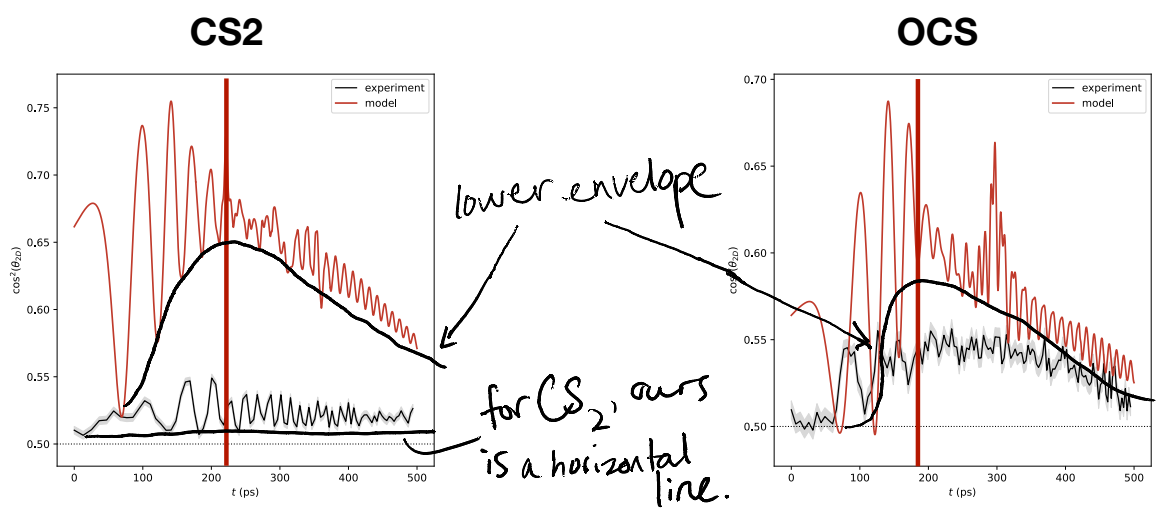
\includegraphics[width=\textwidth]{lower_envelope_comp.png}
\caption*{In reference to Question 3.}
\end{figure}

\clearpage

\begin{figure}
\centering
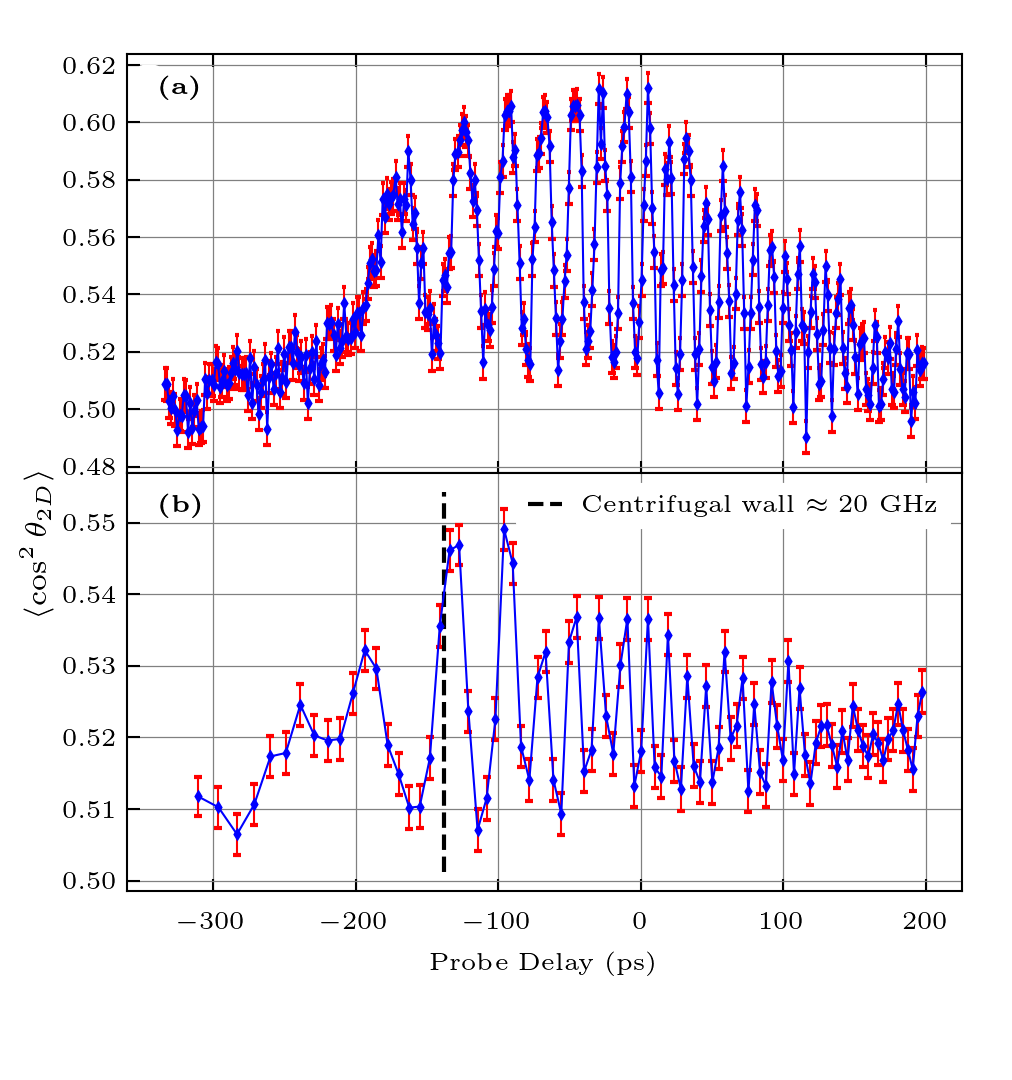
\includegraphics{cs2-breakingwall.png} 
\caption{Molecular alignment of gas-phase CS2 \textbf{(a)} and CS2 molecules embedded in helium droplets \textbf{(b)} to the same phase-stabilized centrifuge. }
\label{cs2_jet_vs_droplet}
\end{figure}
\noindent
\textbf{Comments on figure 1:}
\begin{itemize}
    \item with the centrifuge we are able to spin molecules in helium past the centrifugal wall, which for CS2, is around $20 \, GHz$
    \item compared to the free rotating molecules in the gas-phase there seems to be a decrease in oscillation amplitude after $-100 \, ps$ corresponding to roughly $30-40\, GHz$
\end{itemize}


\begin{figure}[h]
\centering
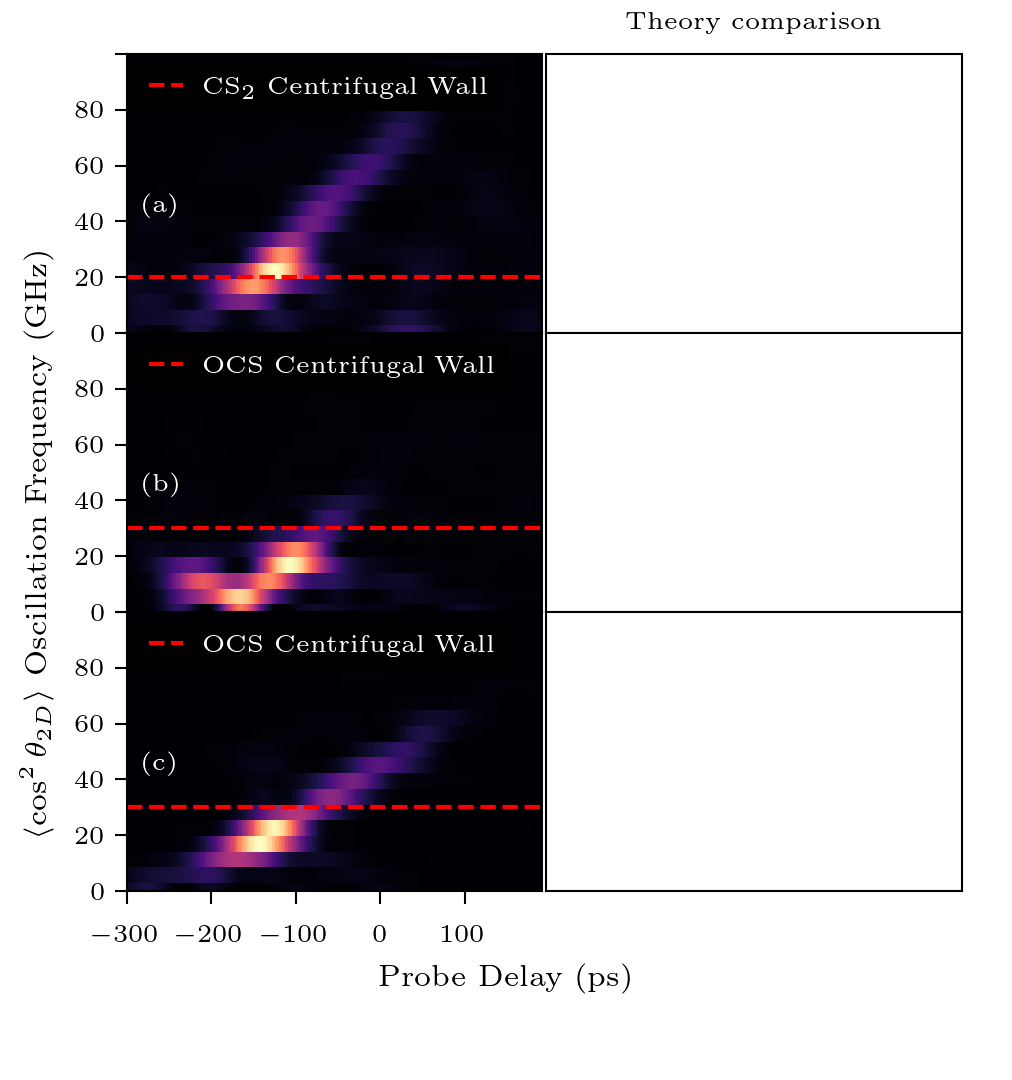
\includegraphics{cs2-ocs-comparison_v1.png}
%\captionsetup{name = Figure 2 [option 1],labelsep=newline}
\caption*{Figure 2 [\textbf{option 1}]: STFT of the experimental (left panel) and theoretical (right panel) $\langle\cos^2\theta_{\mathrm{2D}}\rangle(t)$ signal of molecular rotation in helium droplets of CS\textsubscript{2} \textbf{(a)} and OCS \textbf{(b)} with a higher centrifuge acceleration ($\approx 0.34$ GHz/ps), and OCS \textbf{(c)} with a lower centrifuge acceleration ($\approx 0.26$ GHz/ps). Note that the centrifuge used in \textbf{(b)} decelerates in the beginning of the pulse before reaching 0 GHz and then accelerating. This is reflected in the corresponding spectrogram \textbf{(b)} from about -250 ps to -150 ps.}
\label{cs2_vs_ocs_v1}
\end{figure}
\clearpage
\begin{figure}[h]
\centering
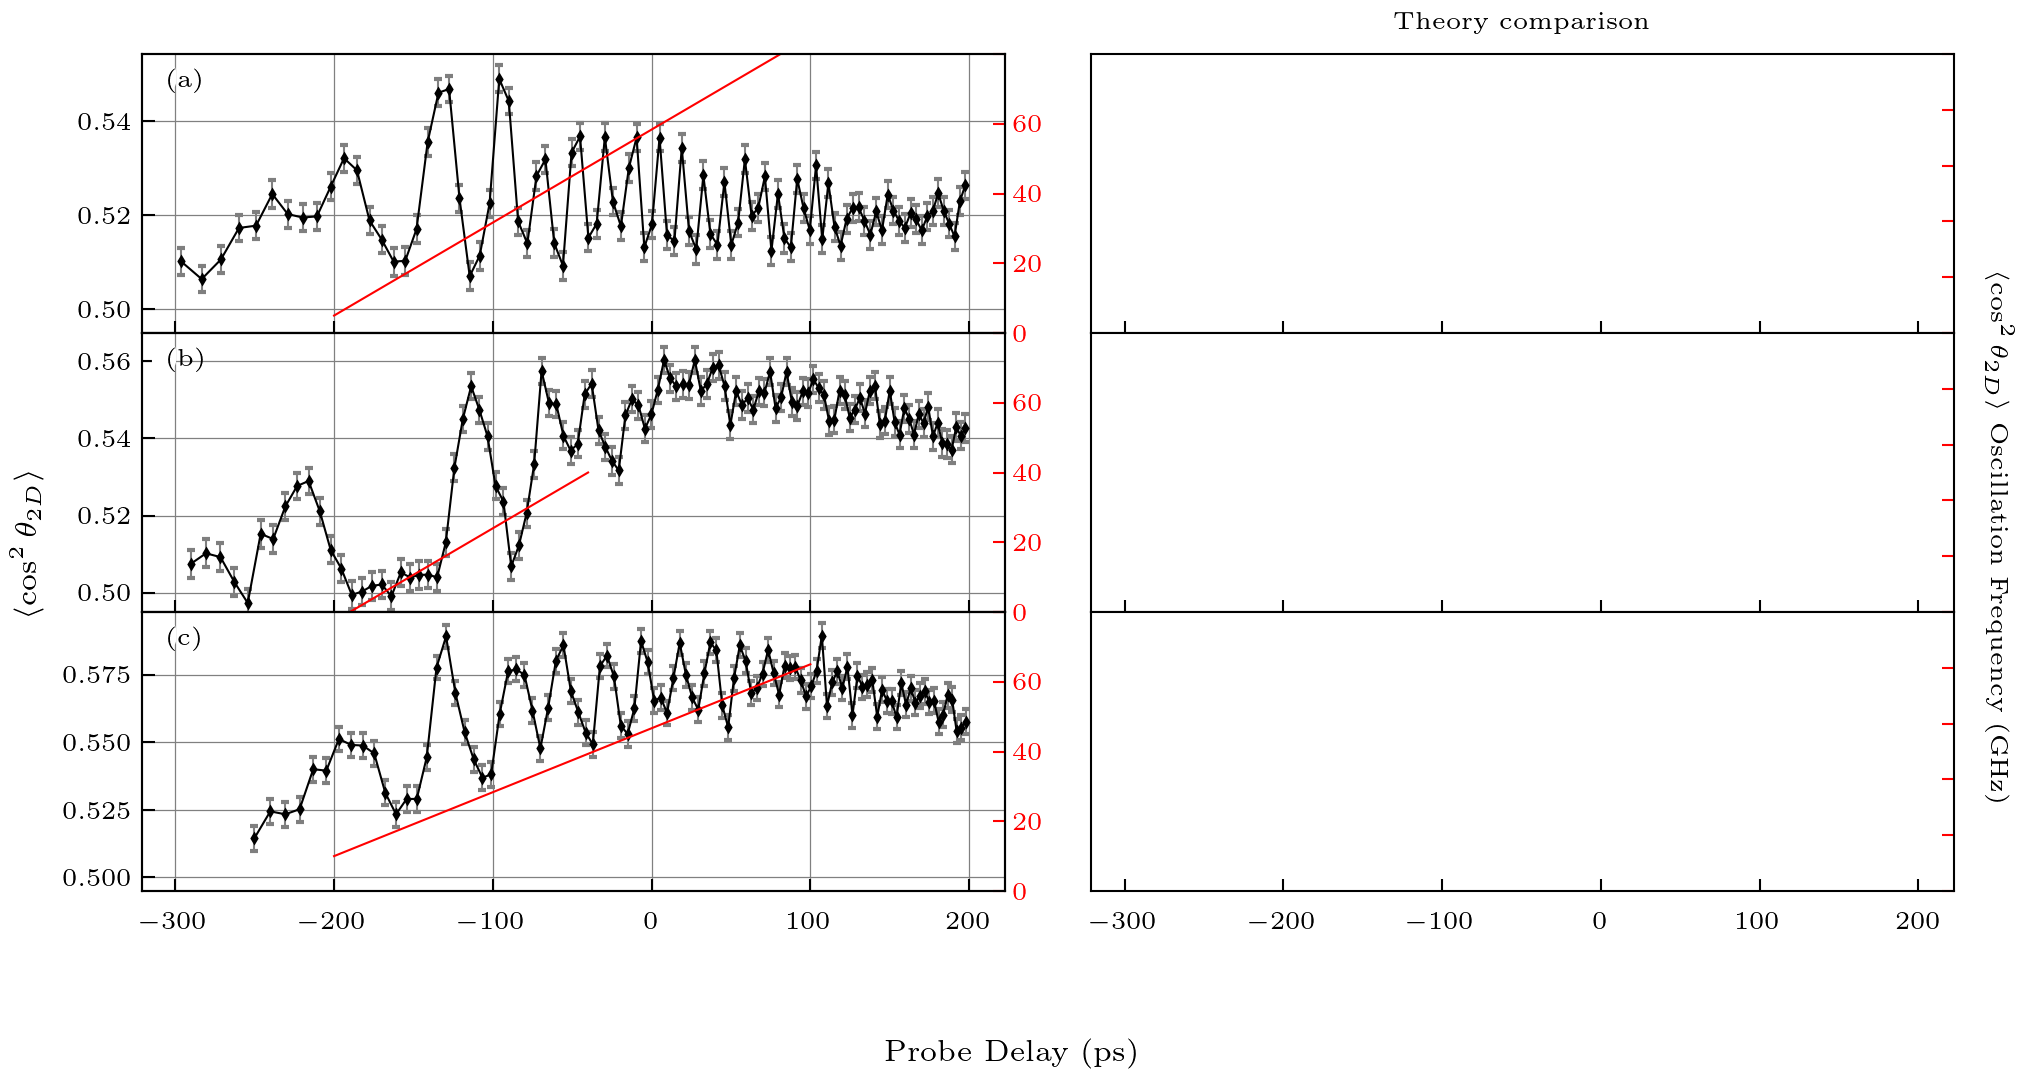
\includegraphics[width=\textwidth]{cs2-ocs-comparison_v2.png}
%\captionsetup{name = Figure 2 [option 2],labelsep=newline}
\caption*{Figure 2 [\textbf{option 2}]: Left panel: Molecular alignment of CS\textsubscript{2} \textbf{(a)} and OCS \textbf{(b)} with a higher centrifuge acceleration ($\approx 0.34$ GHz/ps), and OCS \textbf{(c)} with a lower centrifuge acceleration ($\approx 0.26$ GHz/ps). The truncated lines plotted with respect to the right axes represent the best linear fits (only by eye for now) to the STFTs of the $\langle\cos^2\theta_{\mathrm{2D}}\rangle(t)$ curves. Note that the centrifuge used in \textbf{(b)} decelerates in the beginning of the pulse (-250 ps to -150 ps) before reaching 0 GHz and then accelerating. Right panel: the corresponding theoretical curves and best fit frequency lines.}
\label{cs2_vs_ocs_v3}
\end{figure}


\noindent
\textbf{Comments on figure 2:}
\begin{itemize}
    \item this plot compares two different molecules (CS2 and OCS) and two different centrifuges
    \item we see that in the case of the faster accelerating centrifuge, oscillations persist further for CS2 (a) than OCS (b)
    \item lowering the acceleration makes it possible to see oscillations in OCS (c) until almost $60$ GHz which is again above the centrifugal wall for OCS observed by Henrik's group at around 30 GHz. This partly motivated our question 1 about the dependence on acceleration, as it seems that the ability to spin OCS does indeed improve with lower centrifuge acceleration. 
    \item the comparison to theory should be included in this figure either by plotting the spectrograms (option 1) or by plotting the theoretical $cos^2$ scans (option 2) in the right panels.
\end{itemize}
\end{document}